\begin{table}[htbp]
\centering
\caption{Top 20 venues in Information Retrieval, using P-score and normalized P-score. The suffixes (c) and (j) are used to differentiate conferences and journals with the same name.}
\label{tab:ir-venues}
%\resizebox{\columnwidth}{!}{%
\begin{tabular}{rccc}
\toprule
\#		&	P-score		&	Norm-P-score&	X			\\ \hline
1		&	SIGIR (c)	&	ICTIR		&	SIGIR (c)	\\
2		&	CIKM		&	SIGIR (c)	&	CIKM		\\
3		&	TREC		&	ADCS		&	TREC		\\
4		&	ECIR		&	IR			&	ECIR		\\
5		&	CLEF		&	ECIR		&	CLEF		\\
6		&	WWW			&	TREC		&	SIGIR (j)	\\
7		&	JASIS		&	SIGIR (j)	&	JCDL		\\
8		&	IPM			&	IIIX		&	TOIS		\\
9		&	SIGIR (j)	&	TOIS		&	IR			\\
10		&	MM			&	WSDM		&	WSDM		\\
11		&	JCDL		&	INEX		&	NTCIR		\\
12		&	TOIS		&	SPIRE		&	SPIRE		\\
13		&	IR			&	AIRS		&	AIRS		\\
14		&	WSDM		&	CIKM		&	RIAO		\\
15		&	NTCIR		&	TWEB		&	INEX		\\
16		&	KDD			&	RIAO		&	IIIX		\\
17		&	TKDE		&	CLEF		&	ICTIR		\\
18		&	ACL			&	NTCIR		&	ADCS		\\
19		&	ICDM		&	LA-WEB		&	LA-WEB		\\
20		&	SPIRE		&	JCDL		&	TWEB		\\
\bottomrule

1		&	SIGIR (c)	&	\multirow{20}{*}{\raisebox{-0.9\totalheight}{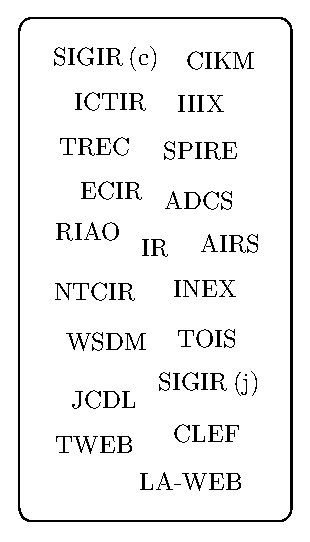
\includegraphics{fig/ir-norm-venues-blob.eps}}}	&	SIGIR (c)	\\ %[width=0.2\textwidth]
2		&	CIKM		&	&	CIKM		\\
3		&	TREC		&	&	TREC		\\
4		&	ECIR		&	&	ECIR		\\
5		&	CLEF		&	&	CLEF		\\
6		&	WWW			&	&	SIGIR (j)	\\
7		&	JASIS		&	&	JCDL		\\
8		&	IPM			&	&	TOIS		\\
9		&	SIGIR (j)	&	&	IR			\\
10		&	MM			&	&	WSDM		\\
11		&	JCDL		&	&	NTCIR		\\
12		&	TOIS		&	&	SPIRE		\\
13		&	IR			&	&	AIRS		\\
14		&	WSDM		&	&	RIAO		\\
15		&	NTCIR		&	&	INEX		\\
16		&	KDD			&	&	IIIX		\\
17		&	TKDE		&	&	ICTIR		\\
18		&	ACL			&	&	ADCS		\\
19		&	ICDM		&	&	LA-WEB		\\
20		&	SPIRE		&	&	TWEB		\\


1		&	SIGIR (c)	\\
2		&	CIKM		\\
3		&	TREC		\\
4		&	ECIR		\\
5		&	CLEF		\\
6		&	SIGIR (j)	\\
7		&	JCDL		\\
8		&	TOIS		\\
9		&	IR			\\
10		&	WSDM		\\
11		&	NTCIR		\\
12		&	SPIRE		\\
13		&	AIRS		\\
14		&	RIAO		\\
15		&	INEX		\\
16		&	IIIX		\\
17		&	ICTIR		\\
18		&	ADCS		\\
19		&	LA-WEB		\\
20		&	TWEB		\\
\end{tabular}
\end{table}

\begin{table}[htbp]
\centering
\caption{Top 20 venues in Databases, using P-score and normalized P-score. The suffixes (c) and (j) are used to differentiate conferences and journals with the same name.}
\label{tab:db-venues}
%\resizebox{\columnwidth}{!}{%
\begin{tabular}{rccc}
\toprule
\#		&		P-score		&		Norm-P-score&		X			\\ \hline
1		&		SIGMOD (c)	&		PVLDB		&		SIGMOD (c)	\\
2		&		ICDE		&		VLDB (j)	&		ICDE		\\
3		&		VLDB (c)	&		CIDR		&		VLDB (c)	\\
4		&		PVLDB		&		SIGMOD (c)	&		PVLDB		\\
5		&		TKDE		&		TODS		&		TKDE		\\
6		&		DEBU		&		DEBU		&		DEBU		\\
7		&		SIGMOD (j)	&		PODS		&		SIGMOD (j)	\\
8		&		EDBT		&		WEBDB		&		EDBT		\\
9		&		CIKM		&		VLDB (c)	&		PODS		\\
10		&		PODS		&		ICDE		&		TODS		\\
11		&		TODS		&		ICDT		&		VLDB (j)	\\
12		&		KDD			&		SIGMOD (j)	&		DASFAA		\\
13		&		VLDB (j)	&		EDBT		&		SSDBM		\\
14		&		WWW			&		SSD			&		ICDT		\\
15		&		ICDM		&		SSDBM		&		CIDR		\\
16		&		DASFAA		&		TKDE		&		WEBDB		\\
17		&		SSDBM		&		DPD			&		SSD			\\
18		&		IS			&		TKDD		&		DPD			\\
19		&		ICDT		&		COMAD		&		COMAD		\\
20		&		CIDR		&		DASFAA		&		TKDD		\\
\bottomrule

\#		&		P-score		&	&		X			\\ \hline
1		&		SIGMOD (c)	&	&		SIGMOD (c)	\\
2		&		ICDE		&	&		ICDE		\\
3		&		VLDB (c)	&	&		VLDB (c)	\\
4		&		PVLDB		&	&		PVLDB		\\
5		&		TKDE		&	&		TKDE		\\
6		&		DEBU		&	&		DEBU		\\
7		&		SIGMOD (j)	&	&		SIGMOD (j)	\\
8		&		EDBT		&	&		EDBT		\\
9		&		CIKM		&	&		PODS		\\
10		&		PODS		&	&		TODS		\\
11		&		TODS		&	&		VLDB (j)	\\
12		&		KDD			&	&		DASFAA		\\
13		&		VLDB (j)	&	&		SSDBM		\\
14		&		WWW			&	&		ICDT		\\
15		&		ICDM		&	&		CIDR		\\
16		&		DASFAA		&	&		WEBDB		\\
17		&		SSDBM		&	&		SSD			\\
18		&		IS			&	&		DPD			\\
19		&		ICDT		&	&		COMAD		\\
20		&		CIDR		&	&		TKDD		\\

\#		&		X			\\ \hline
1		&		SIGMOD (c)	\\
2		&		ICDE		\\
3		&		VLDB (c)	\\
4		&		PVLDB		\\
5		&		TKDE		\\
6		&		DEBU		\\
7		&		SIGMOD (j)	\\
8		&		EDBT		\\
9		&		PODS		\\
10		&		TODS		\\
11		&		VLDB (j)	\\
12		&		DASFAA		\\
13		&		SSDBM		\\
14		&		ICDT		\\
15		&		CIDR		\\
16		&		WEBDB		\\
17		&		SSD			\\
18		&		DPD			\\
19		&		COMAD		\\
20		&		TKDD		\\
\end{tabular}
\end{table}

\begin{table}[htbp]
\centering
\caption{Top 20 venues in Data Mining, using P-score and normalized P-score. The suffixes (c) and (j) are used to differentiate conferences and journals with the same name.}
\label{tab:db-venues}
%\resizebox{\columnwidth}{!}{%
\begin{tabular}{rccc}
    \toprule
\#		&		P-score		&		Norm-P-score&		X			\\ \hline
1		&		KDD			&		TKDD		&		KDD			\\
2		&		ICDM		&		SIGKDD		&		ICDM		\\
3		&		CIKM		&		KDD			&		CIKM		\\
4		&		ICDE		&		SDM			&		ICDE		\\
5		&		ICML		&		DATAMINE	&		ICML		\\
6		&		SDM			&		WSDM		&		SDM			\\
7		&		TKDE		&		ICDM		&		TKDE		\\
8		&		WWW			&		PKDD		&		PKDD		\\
9		&		SIGMOD		&		TIST		&		PAKDD		\\
10		&		AAAI		&		SADM		&		SIGKDD		\\
11		&		PKDD		&		KAIS		&		DATAMINE	\\
12		&		NIPS		&		PAKDD		&		KAIS		\\
13		&		PAKDD		&		TKDE		&		PVLDB		\\
14		&		VLDB (c)	&		ICML		&		WSDM		\\
15		&		SIGIR		&		VLDB (c)	&		TKDD		\\
16		&		SIGKDD		&		CIKM		&		VLDB (c)	\\
17		&		DATAMINE	&		SSD			&		RECSYS		\\
18		&		KAIS		&		RECSYS		&		TIST		\\
19		&		JMLR		&		ICDE		&		SSD			\\
20		&		PVLDB		&		PVLDB		&		SADM		\\
\bottomrule

\#		&		P-score		& &		X			\\ \hline
1		&		KDD			& &		KDD			\\
2		&		ICDM		& &		ICDM		\\
3		&		CIKM		& &		CIKM		\\
4		&		ICDE		& &		ICDE		\\
5		&		ICML		& &		ICML		\\
6		&		SDM			& &		SDM			\\
7		&		TKDE		& &		TKDE		\\
8		&		WWW			& &		PKDD		\\
9		&		SIGMOD		& &		PAKDD		\\
10		&		AAAI		& &		SIGKDD		\\
11		&		PKDD		& &		DATAMINE	\\
12		&		NIPS		& &		KAIS		\\
13		&		PAKDD		& &		PVLDB		\\
14		&		VLDB (c)	& &		WSDM		\\
15		&		SIGIR		& &		TKDD		\\
16		&		SIGKDD		& &		VLDB (c)	\\
17		&		DATAMINE	& &		RECSYS		\\
18		&		KAIS		& &		TIST		\\
19		&		JMLR		& &		SSD			\\
20		&		PVLDB		& &		SADM		\\

1		&		KDD			\\
2		&		ICDM		\\
3		&		CIKM		\\
4		&		ICDE		\\
5		&		ICML		\\
6		&		SDM			\\
7		&		TKDE		\\
8		&		PKDD		\\
9		&		PAKDD		\\
10		&		SIGKDD		\\
11		&		DATAMINE	\\
12		&		KAIS		\\
13		&		PVLDB		\\
14		&		WSDM		\\
15		&		TKDD		\\
16		&		VLDB (c)	\\
17		&		RECSYS		\\
18		&		TIST		\\
19		&		SSD			\\
20		&		SADM		\\

\end{tabular}
\end{table}














\begin{table}[htbp]
\centering
\caption{Top 20 venues in Databases, using (i) standard P-score, (ii) normalized P-score, and (iii) re-ranking the set of venues obtained in (ii) according to their P-scores. The suffixes (c) and (j) are used to differentiate conferences and journals with the same name.}
\label{tab:db-venues}
%\resizebox{\columnwidth}{!}{%
\begin{tabular}{rc}
\toprule
\#		&	Standard P-score \\ 
\midrule
1		&		SIGMOD (c)	\\
2		&		ICDE		\\
3		&		VLDB (c)	\\
4		&		PVLDB		\\
5		&		TKDE		\\
6		&		DEBU		\\
7		&		SIGMOD (j)	\\
8		&		EDBT		\\
9		&		CIKM		\\
10		&		PODS		\\
11		&		TODS		\\
12		&		KDD			\\
13		&		VLDB (j)	\\
14		&		WWW			\\
15		&		ICDM		\\
16		&		DASFAA		\\
17		&		SSDBM		\\
18		&		IS			\\
19		&		ICDT		\\
20		&		CIDR		\\
\bottomrule
\end{tabular} \ \ 
\begin{tabular}{c}
\toprule
norm-P-score \\ 
\midrule
%\vspace{-30px}
\multirow{20}{*}{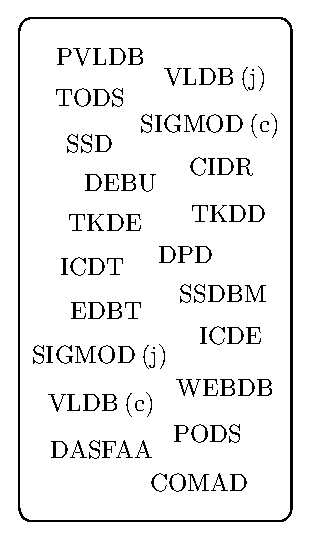
\includegraphics{fig/db-norm-venues-blob.eps}} \\ %[width=0.2\linewidth]
\\
\\
\\
\\
\\
\\
\\
\\
\\
\\
\\
\\
\\
\\
\\
\\
\\
\\
\\
\bottomrule
\end{tabular} \ \
\begin{tabular}{rc}
\toprule
\#		&	Final Ranking \\ 
\midrule
1		&		SIGMOD (c)	\\
2		&		ICDE		\\
3		&		VLDB (c)	\\
4		&		PVLDB		\\
5		&		TKDE		\\
6		&		DEBU		\\
7		&		SIGMOD (j)	\\
8		&		EDBT		\\
9		&		PODS		\\
10		&		TODS		\\
11		&		VLDB (j)	\\
12		&		DASFAA		\\
13		&		SSDBM		\\
14		&		ICDT		\\
15		&		CIDR		\\
16		&		WEBDB		\\
17		&		SSD			\\
18		&		DPD			\\
19		&		COMAD		\\
20		&		TKDD		\\
\bottomrule
\end{tabular}
\end{table}

\begin{table}[htbp]
\centering
\caption{Top 20 venues in Data Mining, using (i) standard P-score, (ii) normalized P-score, and (iii) re-ranking the set of venues obtained in (ii) according to their P-scores. The suffixes (c) and (j) are used to differentiate conferences and journals with the same name.}
\label{tab:dm-venues}
%\resizebox{\columnwidth}{!}{%
\begin{tabular}{rc}
\toprule
\#		&	Standard P-score \\ 
\midrule
1		&		KDD			\\
2		&		ICDM		\\
3		&		CIKM		\\
4		&		ICDE		\\
5		&		ICML		\\
6		&		SDM			\\
7		&		TKDE		\\
8		&		WWW			\\
9		&		SIGMOD		\\
10		&		AAAI		\\
11		&		PKDD		\\
12		&		NIPS		\\
13		&		PAKDD		\\
14		&		VLDB (c)	\\
15		&		SIGIR		\\
16		&		SIGKDD		\\
17		&		DATAMINE	\\
18		&		KAIS		\\
19		&		JMLR		\\
20		&		PVLDB		\\
\bottomrule
\end{tabular} \ \ 
\begin{tabular}{c}
\toprule
norm-P-score \\ 
\midrule
%\vspace{-30px}
\multirow{20}{*}{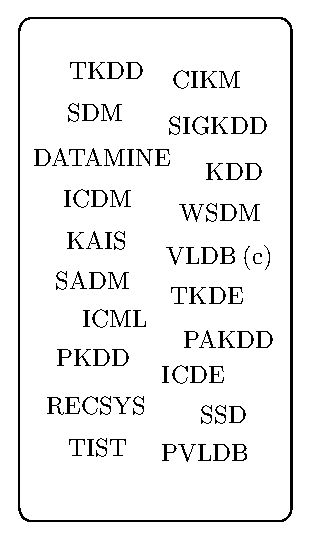
\includegraphics{fig/dm-norm-venues-blob.eps}} \\ %[width=0.2\linewidth]
\\
\\
\\
\\
\\
\\
\\
\\
\\
\\
\\
\\
\\
\\
\\
\\
\\
\\
\\
\bottomrule
\end{tabular} \ \
\begin{tabular}{rc}
\toprule
\#		&	Final Ranking \\ 
\midrule
1		&		KDD			\\
2		&		ICDM		\\
3		&		CIKM		\\
4		&		ICDE		\\
5		&		ICML		\\
6		&		SDM			\\
7		&		TKDE		\\
8		&		PKDD		\\
9		&		PAKDD		\\
10		&		SIGKDD		\\
11		&		DATAMINE	\\
12		&		KAIS		\\
13		&		PVLDB		\\
14		&		WSDM		\\
15		&		TKDD		\\
16		&		VLDB (c)	\\
17		&		RECSYS		\\
18		&		TIST		\\
19		&		SSD			\\
20		&		SADM		\\
\bottomrule
\end{tabular}
\end{table}

















%\raisebox{-\totalheight}{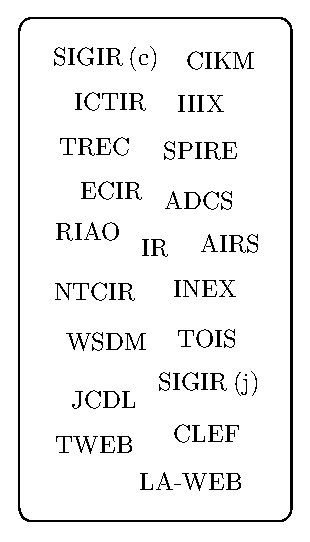
\includegraphics[width=0.3\textwidth]{fig/ir-norm-venues-blob.eps}} 

\begin{table}[htbp]
\centering
\caption{Top 20 venues in Information Retrieval, using (i) standard P-score, (ii) normalized P-score, and (iii) re-ranking the set of venues obtained in (ii) according to their P-scores. The suffixes (c) and (j) are used to differentiate conferences and journals with the same name.}
\label{tab:ir-venues}
%\resizebox{\columnwidth}{!}{%
\begin{tabular}{rccc}
\toprule
\#		&	Standard P-score		&	Norm-P-score 	&	Final Ranking 			\\ 
\midrule
1		&	SIGIR (c)	&	\multirow{20}{*}{\raisebox{-0.9\totalheight}{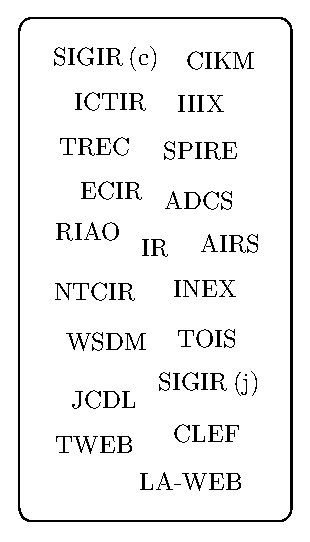
\includegraphics{fig/ir-norm-venues-blob.eps}}}	&	SIGIR (c)	\\ %[width=0.2\textwidth]
2		&	CIKM		&	&	CIKM		\\
3		&	TREC		&	&	TREC		\\
4		&	ECIR		&	&	ECIR		\\
5		&	CLEF		&	&	CLEF		\\
6		&	WWW			&	&	SIGIR (j)	\\
7		&	JASIS		&	&	JCDL		\\
8		&	IPM			&	&	TOIS		\\
9		&	SIGIR (j)	&	&	IR			\\
10		&	MM			&	&	WSDM		\\
11		&	JCDL		&	&	NTCIR		\\
12		&	TOIS		&	&	SPIRE		\\
13		&	IR			&	&	AIRS		\\
14		&	WSDM		&	&	RIAO		\\
15		&	NTCIR		&	&	INEX		\\
16		&	KDD			&	&	IIIX		\\
17		&	TKDE		&	&	ICTIR		\\
18		&	ACL			&	&	ADCS		\\
19		&	ICDM		&	&	LA-WEB		\\
20		&	SPIRE		&	&	TWEB		\\
\bottomrule
\end{tabular}
\end{table}


\begin{table}[htbp]
\centering
\caption{Top 20 venues in Databases, using (i) standard P-score, (ii) normalized P-score, and (iii) re-ranking the set of venues obtained in (ii) according to their P-scores. The suffixes (c) and (j) are used to differentiate conferences and journals with the same name.}
\label{tab:db-venues}
%\resizebox{\columnwidth}{!}{%
\begin{tabular}{rccc}
\toprule
\#		&	Standard P-score		&	Norm-P-score 	&	Final Ranking 			\\
\midrule 
1		&		SIGMOD (c)	&	\multirow{20}{*}{\raisebox{-0.9\totalheight}{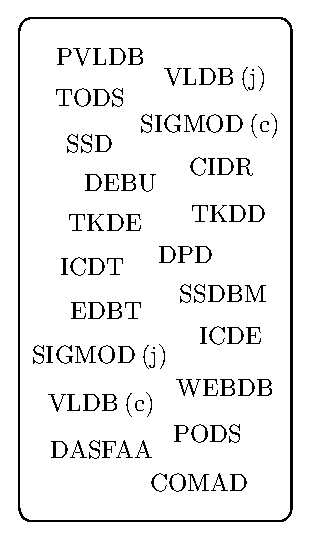
\includegraphics{fig/db-norm-venues-blob.eps}}}	&		SIGMOD (c)	\\
2		&		ICDE		&	&		ICDE		\\
3		&		VLDB (c)	&	&		VLDB (c)	\\
4		&		PVLDB		&	&		PVLDB		\\
5		&		TKDE		&	&		TKDE		\\
6		&		DEBU		&	&		DEBU		\\
7		&		SIGMOD (j)	&	&		SIGMOD (j)	\\
8		&		EDBT		&	&		EDBT		\\
9		&		CIKM		&	&		PODS		\\
10		&		PODS		&	&		TODS		\\
11		&		TODS		&	&		VLDB (j)	\\
12		&		KDD			&	&		DASFAA		\\
13		&		VLDB (j)	&	&		SSDBM		\\
14		&		WWW			&	&		ICDT		\\
15		&		ICDM		&	&		CIDR		\\
16		&		DASFAA		&	&		WEBDB		\\
17		&		SSDBM		&	&		SSD			\\
18		&		IS			&	&		DPD			\\
19		&		ICDT		&	&		COMAD		\\
20		&		CIDR		&	&		TKDD		\\
\bottomrule
\end{tabular}
\end{table}

\begin{table}[htbp]
\centering
\caption{Top 20 venues in Data Mining, using (i) standard P-score, (ii) normalized P-score, and (iii) re-ranking the set of venues obtained in (ii) according to their P-scores. The suffixes (c) and (j) are used to differentiate conferences and journals with the same name.}
\label{tab:dm-venues}
%\resizebox{\columnwidth}{!}{%
\begin{tabular}{rccc}
\toprule
\#		&	Standard P-score		&	Norm-P-score 	&	Final Ranking 			\\ 
\midrule
1		&		KDD			& \multirow{20}{*}{\raisebox{-0.9\totalheight}{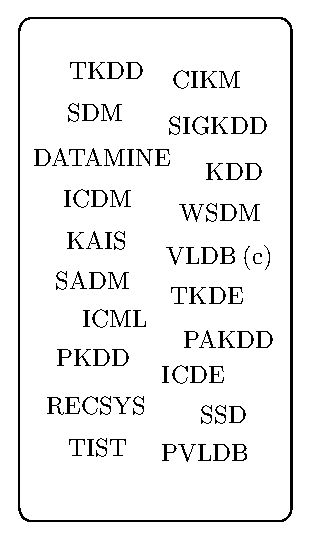
\includegraphics{fig/dm-norm-venues-blob.eps}}}	&		KDD			\\
2		&		ICDM		& &		ICDM		\\
3		&		CIKM		& &		CIKM		\\
4		&		ICDE		& &		ICDE		\\
5		&		ICML		& &		ICML		\\
6		&		SDM			& &		SDM			\\
7		&		TKDE		& &		TKDE		\\
8		&		WWW			& &		PKDD		\\
9		&		SIGMOD		& &		PAKDD		\\
10		&		AAAI		& &		SIGKDD		\\
11		&		PKDD		& &		DATAMINE	\\
12		&		NIPS		& &		KAIS		\\
13		&		PAKDD		& &		PVLDB		\\
14		&		VLDB (c)	& &		WSDM		\\
15		&		SIGIR		& &		TKDD		\\
16		&		SIGKDD		& &		VLDB (c)	\\
17		&		DATAMINE	& &		RECSYS		\\
18		&		KAIS		& &		TIST		\\
19		&		JMLR		& &		SSD			\\
20		&		PVLDB		& &		SADM		\\
\bottomrule
\end{tabular}
\end{table}

It is noteworthy to mention that the normalized P-score ranking of venues should not be interpreted as an impact or productivity ranking. We only use this output to define the most representative venues of a subarea, in a semi-automatic fashion. {\color{blue} For this reason, in Tables~\ref{tab:ir-venues},~\ref{tab:db-venues}, and~\ref{tab:dm-venues}, we present the results obtained by normalized P-scores as sets of venues instead of rankings of venues.}













\begin{tabular}{rc}
\toprule
\#		&	Standard P-score \\ 
\midrule
1		&	SIGIR (c) \\
2		&	CIKM		\\
3		&	TREC	\\	
4		&	ECIR		\\
5		&	CLEF		\\
6		&	WWW	\\		
7		&	JASIS	\\	
8		&	IPM		\\	
9		&	SIGIR (j) \\
10		&	MM	\\		
11		&	JCDL		\\
12		&	TOIS		\\
13		&	IR			\\
14		&	WSDM	\\
15		&	NTCIR	\\
16		&	KDD		\\
17		&	TKDE	\\
18		&	ACL		\\
19		&	ICDM		\\
20		&	SPIRE	\\
\bottomrule
\end{tabular} \ \ 
\begin{tabular}{c}
\toprule
norm-P-score \\ 
\midrule
%\vspace{-30px}
\multirow{20}{*}{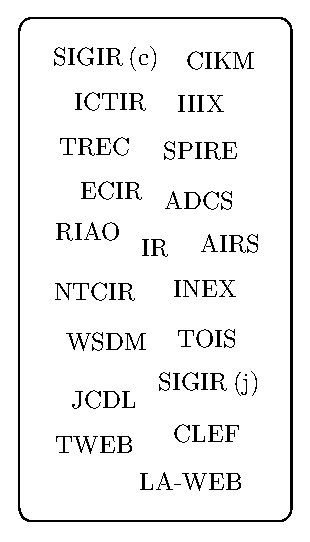
\includegraphics{fig/ir-norm-venues-blob.eps}} \\ %[width=0.2\linewidth]
\\
\\
\\
\\
\\
\\
\\
\\
\\
\\
\\
\\
\\
\\
\\
\\
\\
\\
\\
\bottomrule
\end{tabular} \ \
\begin{tabular}{rc}
\toprule
\#		&	Final Ranking \\ 
\midrule
1		&	SIGIR (c)	\\
2		&	CIKM		\\
3		&	TREC		\\
4		&	ECIR		\\
5		&	CLEF		\\
6		&	SIGIR (j)	\\
7		&	JCDL		\\
8		&	TOIS		\\
9		&	IR			\\
10		&	WSDM		\\
11		&	NTCIR		\\
12		&	SPIRE		\\
13		&	AIRS		\\
14		&	RIAO		\\
15		&	INEX		\\
16		&	IIIX		\\
17		&	ICTIR		\\
18		&	ADCS		\\
19		&	LA-WEB		\\
20		&	TWEB		\\

\bottomrule
\end{tabular}
